\section{Properties of CoT-ICL}

\subsection{Scaling with Reasoning Tasks}
\label{sec:scalingtasks}
Prior work reports that many-shot ICL yields reliable improvements on non-reasoning tasks~\cite{bertsch-etal-2025-context, baek2025revisitingincontextlearninglong}. We replicate this behavior, but find it does \emph{not} extend to reasoning tasks when demonstrations include CoT rationales.
Figure~\ref{fig:overview} shows a clear contrast: non-reasoning tasks improve steadily as the number of demonstrations increases, whereas reasoning performance is unstable and often degrades for non-reasoning LLMs.

This failure is not explained by insufficient parameter scale.
As shown in Figure~\ref{fig:llama70} (left), even Llama~3.3~70B can incur negative gains from adding more CoT demonstrations.
Together, these results suggest a qualitative difference between scaling traditional ICL and CoT-ICL.




\begin{figure}[t!]
    \centering
    \begin{subfigure}[b]{\linewidth}
        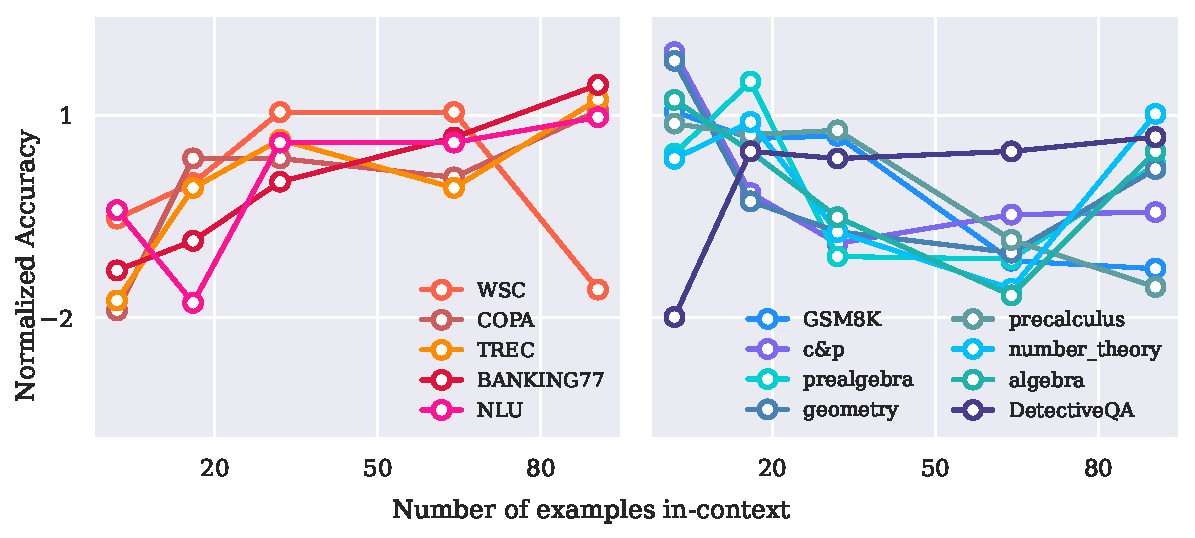
\includegraphics[width=\linewidth]{figures/llama3.1_7b.pdf}
        \caption{Llama-3.1-8B-Instruct}
    \end{subfigure}
    \hfill
    \begin{subfigure}[b]{\linewidth}
        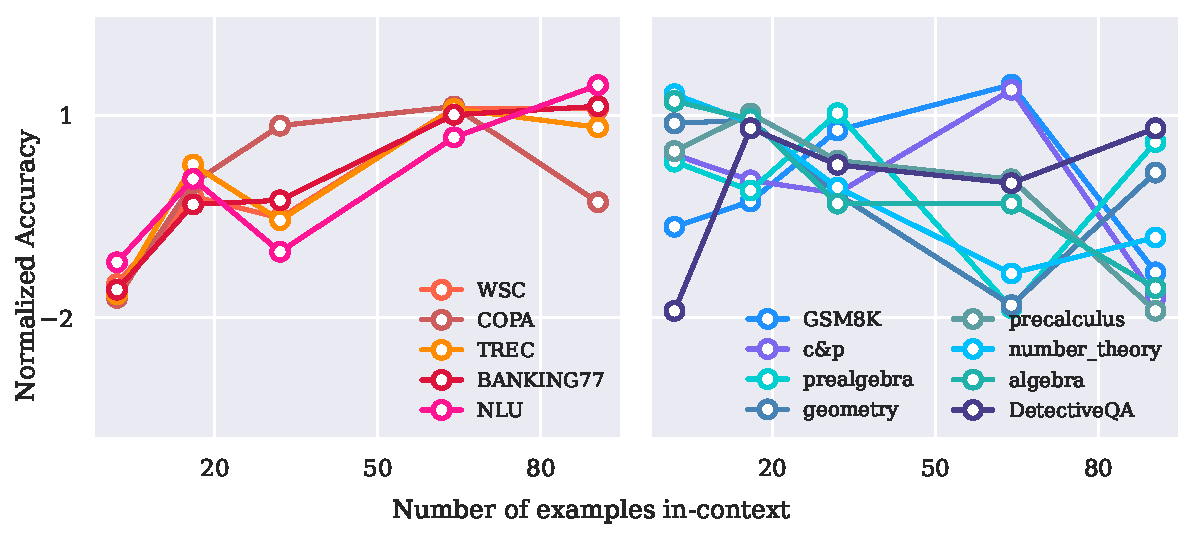
\includegraphics[width=\linewidth]{figures/qwen2.5_7b.pdf}
        \caption{Qwen2.5-7B-Instruct}
    \end{subfigure}
    \hfill
    \begin{subfigure}[b]{\linewidth}
        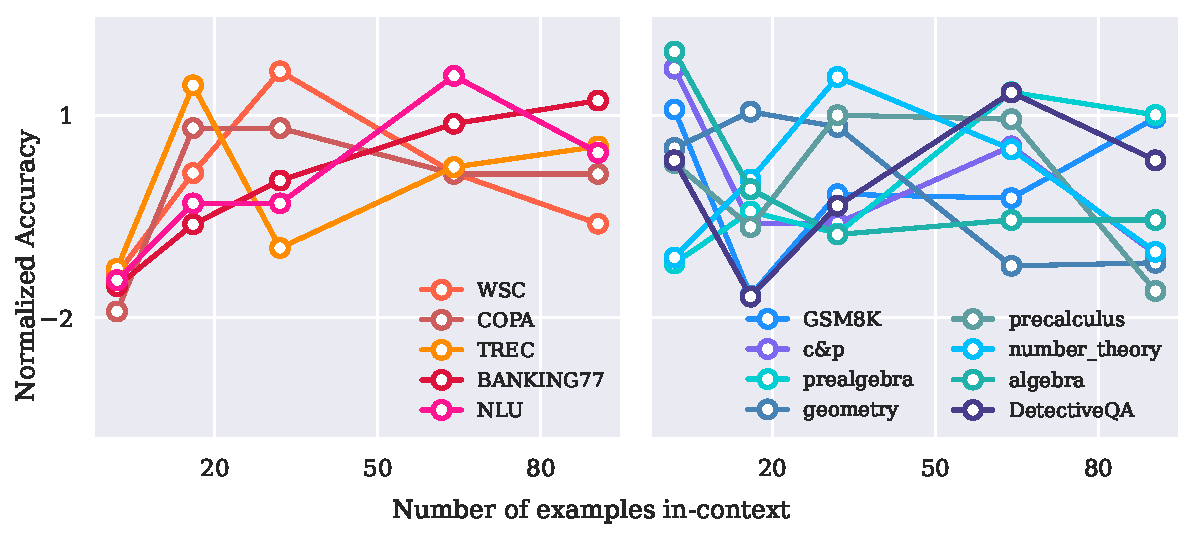
\includegraphics[width=\linewidth]{figures/qwen2.5_14b.pdf}
        \caption{Qwen2.5-14B-Instruct}
    \end{subfigure}
    \caption{Scaling disparity between task types. Performance (normalized accuracy) of non-reasoning LLMs on classification tasks (\textcolor{orange}{warm colors}) versus reasoning tasks (\textcolor{Cerulean}{cool colors}). The x-axis represents normalized accuracy (i.e., $\frac{x-\bar{x}}{\sigma_x}$ for accuracy $x$), while the y-axis indicates the number of in-context demonstrations.}
    \label{fig:overview}
    \vspace{-1mm}
\end{figure}


\begin{figure}[t!]
    \centering
    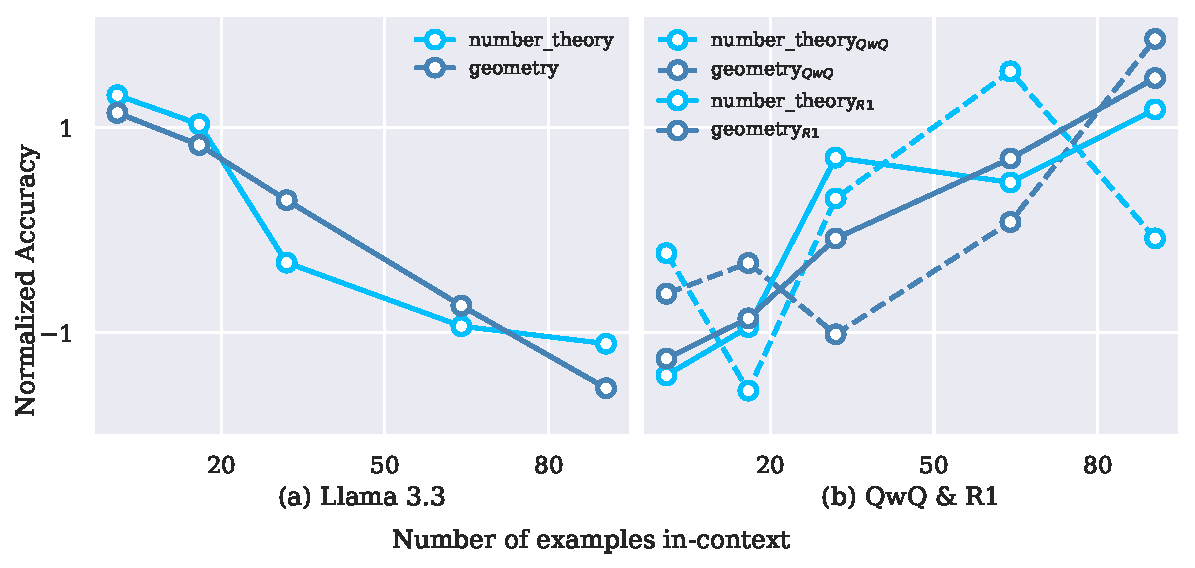
\includegraphics[width=\linewidth]{figures/combined_plot.pdf}
        \caption{Scaling disparity between model types on math reasoning tasks. \emph{Left:} Llama 3.3 (non-reasoning LLM) shows negative gains. \emph{Right:} QwQ (32B) and R1 (685 B)  (reasoning LLM) shows clear positive scaling.}
    \label{fig:llama70}
\end{figure}

\subsection{Scaling with Reasoning LLMs}
\label{sec:scalingllms}

The scaling behavior changes markedly for models with explicit reasoning capabilities.
Figure~\ref{fig:llama70} (right) shows that QwQ~(32B) and R1 (685B) improves consistently as more CoT demonstrations are added.
This trend also holds for smaller reasoning-optimized models: across the Qwen3 family (Figure~\ref{fig:qwen3}), performance increases near-monotonically with additional demonstrations.

The divergence between model classes indicates that benefiting from long CoT contexts is not a generic consequence of having more examples in context.
Instead, positive scaling appears to require model mechanisms that can use demonstrations as intermediate reasoning signal (e.g., via thinking tokens and/or reasoning-oriented training), rather than relying primarily on shallow pattern matching.
To directly test this interpretation, we evaluate the same $n=128$ many-shot CoT contexts with thinking enabled versus disabled. As shown in Table~\ref{tab:thinking_ablation_main}, suppressing the generation of intermediate reasoning hurts performance on geometry and number\_theory for both Qwen3 models, and also hurts DetectiveQA for Qwen3-8B. Furthermore, when thinking is enabled on geometry, increasing $n$ from 16 to 128 improves Qwen3-14B accuracy from 66.18\% to 73.07\%, while reducing the average number of generated tokens inside the \texttt{<think>} segment by 24.02\%. This suggests that larger CoT contexts help the model internalize task procedures, reducing the need for verbose query-time deliberation.

\begin{table}[t]
\centering
\resizebox{0.95\columnwidth}{!}{
\begin{tabular}{lccc}
\toprule
Model & geometry & number\_theory & DetectiveQA \\ \midrule
Qwen3-14B (en) & \textbf{73.07} & \textbf{91.30} & 72.73 \\
Qwen3-14B (dis) & 65.76 & 88.15 & 72.73 \\
Qwen3-8B (en) & \textbf{67.01} & \textbf{84.63} & \textbf{69.48} \\
Qwen3-8B (dis) & 62.63 & 79.81 & 66.88 \\ \bottomrule
\end{tabular}
}
\caption{Performance at $n=128$ with reasoning-oriented models' thinking mode \textbf{(en)}abled versus \textbf{(dis)}abled.}
\label{tab:thinking_ablation_main}
\vspace{-7mm}
\end{table}


\begin{figure}[t!]
    \centering
    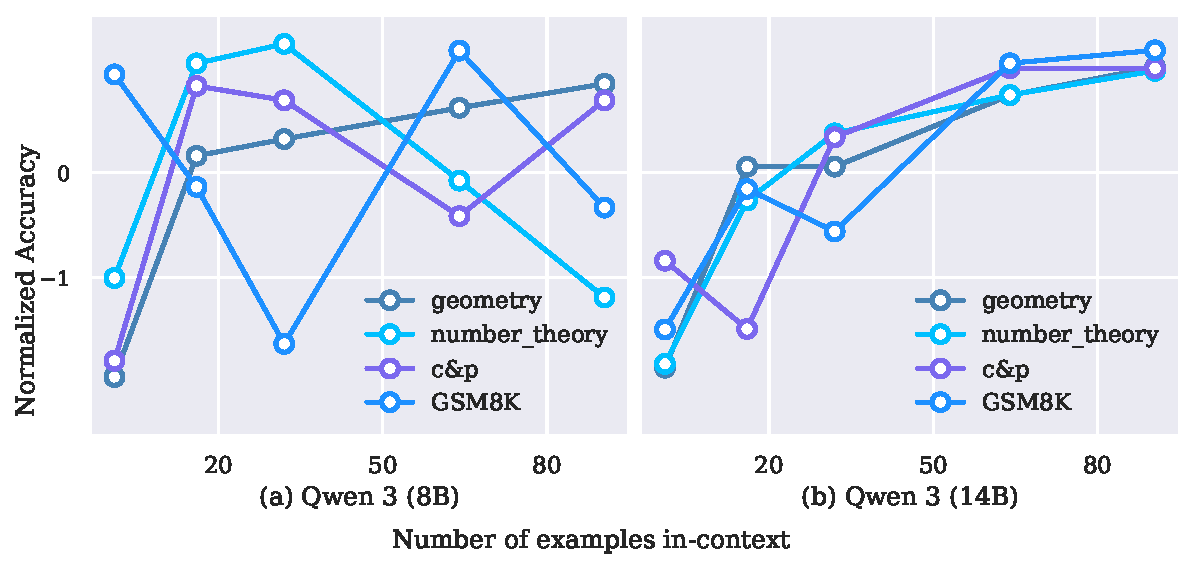
\includegraphics[width=\linewidth]{figures/qwen314.pdf}
    \caption{Positive scaling of reasoning LLMs. The Qwen3 family (reasoning LLMs) demonstrates consistent performance improvements with more demonstrations on math reasoning tasks. \emph{Left:} Qwen3 (8B) \emph{Right:} Qwen3 (14B)}
    \label{fig:qwen3}
    \vspace{-1mm}
\end{figure}

\subsection{Rethinking ICL with similarity} 
\label{sec:sim}

Sections~\ref{sec:scalingtasks}--\ref{sec:scalingllms} reveal a consistent split: many-shot ICL scales reliably on non-reasoning tasks, while many-shot CoT-ICL for reasoning is unstable for non-reasoning LLMs and improves mainly for reasoning-optimized LLMs.

For positive scaling effect, a common explanation for why many-shot ICL works is the \emph{retrieval hypothesis}: additional demonstrations help because the model can locate and reuse examples that are semantically similar to the query~\cite{liu-etal-2022-makes, wu-etal-2023-self}.
If many-shot CoT-ICL for reasoning were driven by the same mechanism, then (i) retrieving question-similar demonstrations should help more as $k$ grows, and (ii) the most-similar set should consistently outperform dissimilar or uncurated sets.

For each test query, we embed all candidate \emph{training questions} (question-only) with Qwen3-Embedding-4B~\cite{zhang2025qwen3embeddingadvancingtext} and rank candidates by cosine similarity.
We then build two $k$-shot demonstration sets per query: (i) \emph{most-similar} (top-$k$) and (ii) \emph{most-dissimilar} (bottom-$k$), keeping the original CoT+answer paired with each selected question.
We evaluate five base LLMs (Llama~3.1, Qwen~2.5 7B/14B, Qwen3 8B/14B) and report averages; details are in Appendix~\ref{sec:sim_setup}.

\emph{Similarity retrieval succeeds for non-reasoning tasks, but fails for reasoning tasks.}
Figure~\ref{fig:sim} supports the retrieval hypothesis on a non-reasoning task BANKING77. The most-similar sets consistently outperform the most-dissimilar sets.
However, the same heuristic breaks on reasoning tasks.
Across geometry, number\_theory, and DetectiveQA, the most-similar sets are consistently \emph{worse} than either the most-dissimilar sets or the original (unretrieved) sets.
This conclusion holds when evaluating reasoning and non-reasoning LLMs separately (Appendix~\ref{sec:simdis_reasoningornot}).

\emph{Similarity optimizes matching, not learning.}
These results align with the paper's central message: many-shot CoT-ICL for reasoning is not well explained as scaled-up pattern matching.
For non-reasoning tasks, question-level similarity is often a reliable proxy for label similarity, so retrieving similar demonstrations improves performance.
For reasoning tasks, in contrast, question-level similarity is a weak proxy for procedural compatibility. Two problems can look semantically similar while requiring different solution strategies, and their associated CoT-ICL may induce conflicting intermediate steps. We provide qualitative examples and additional analysis in Appendix~\ref{sec:sim_qual}.

This provides a mechanism-level explanation for the negative scaling observed in Section~\ref{sec:scalingtasks}.
Solving reasoning tasks depends on extracting and reusing \emph{procedures}, not merely matching surface patterns. With purely surface matching and LLMs are likely to be misled by a set of ``similar'' but procedurally mismatched CoTs, leading to negative gains with similar retrieval.

The failure of similarity-based retrieval with reasoning LLMs also suggests that the mechanism behind positive scaling differs across settings.
In particular, the rationale for why scaling works for reasoning-oriented LLMs on reasoning tasks (Section~\ref{sec:scalingllms}) is not the same as why scaling works for non-reasoning LLMs on non-reasoning tasks (Section~\ref{sec:scalingtasks}).
From a learning perspective, a plausible explanation is that reasoning-oriented models can better interpret the provided CoT-ICL and extract higher-level procedural structure in the thinking content beyond surface pattern matching, allowing the benefit from additional demonstrations.










\begin{figure}[t]
    \centering
    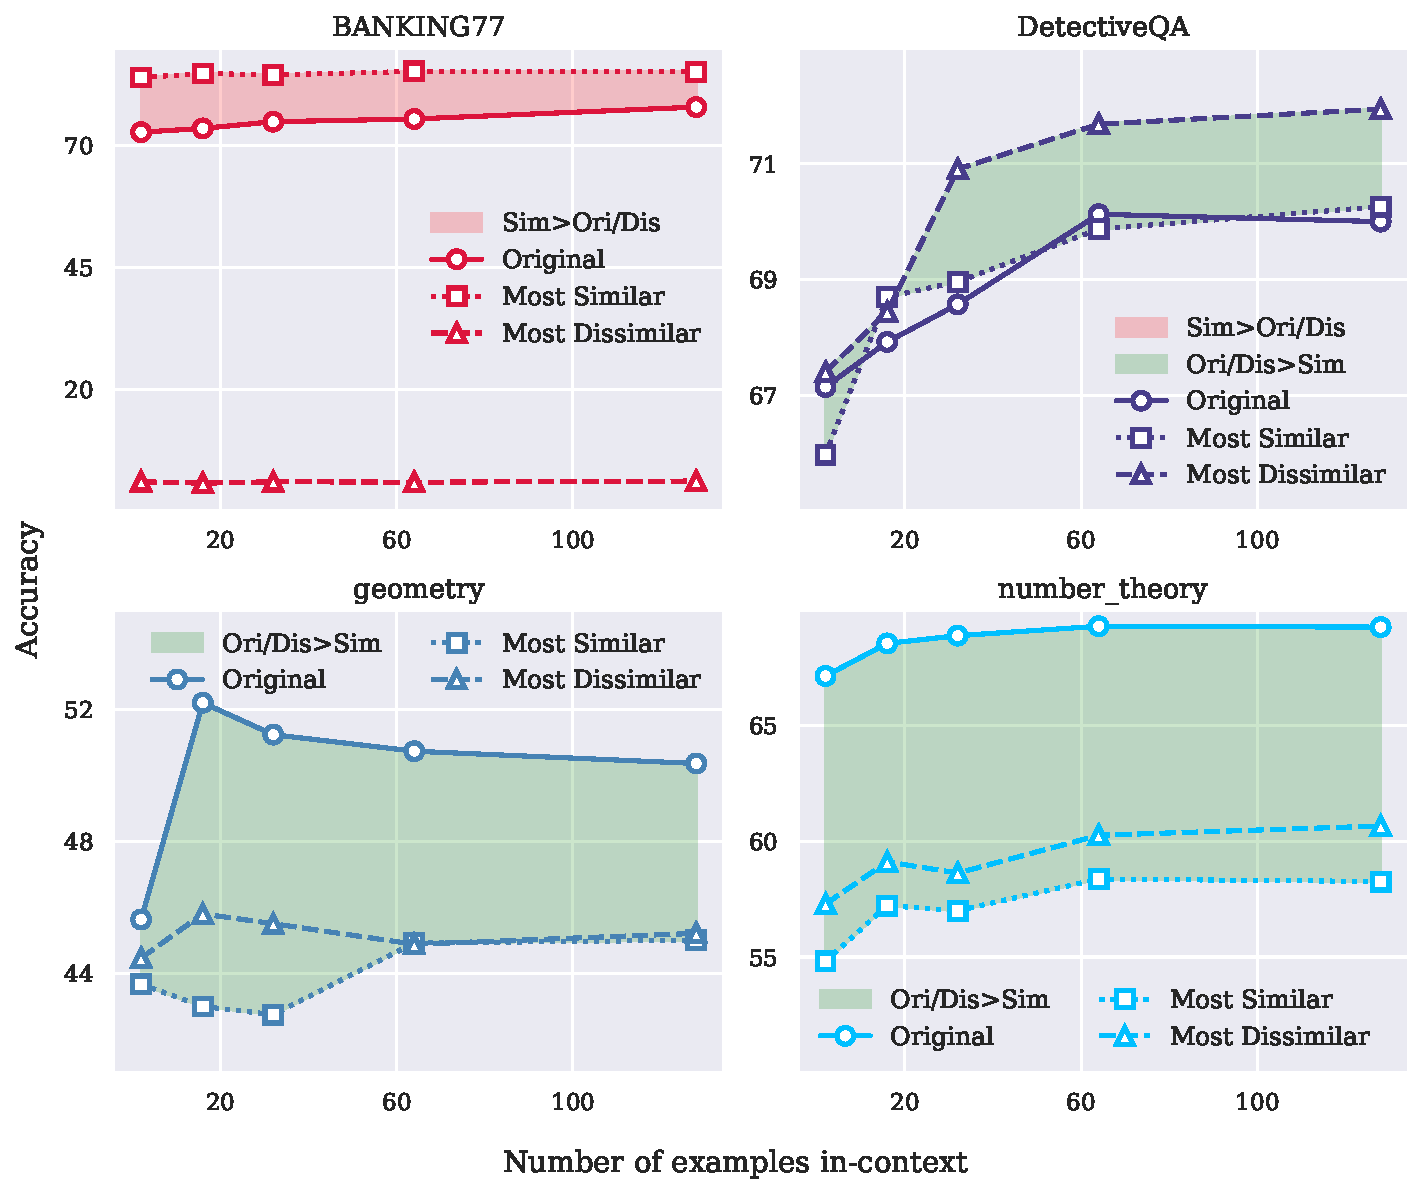
\includegraphics[width=\linewidth]{figures/similarity.pdf}
    \caption{Performance with original(ori), similarity(sim) and dissimilar(dis) sets averaged across five LLMs. The area between the two sets is filled with colors, indicating the relative performance.}
    \label{fig:sim}
\end{figure}









\subsection{Ordering Stability of CoT-ICL}
\label{sec:variance}


 \begin{figure}[t]
    \centering
    \vspace{-2mm}
    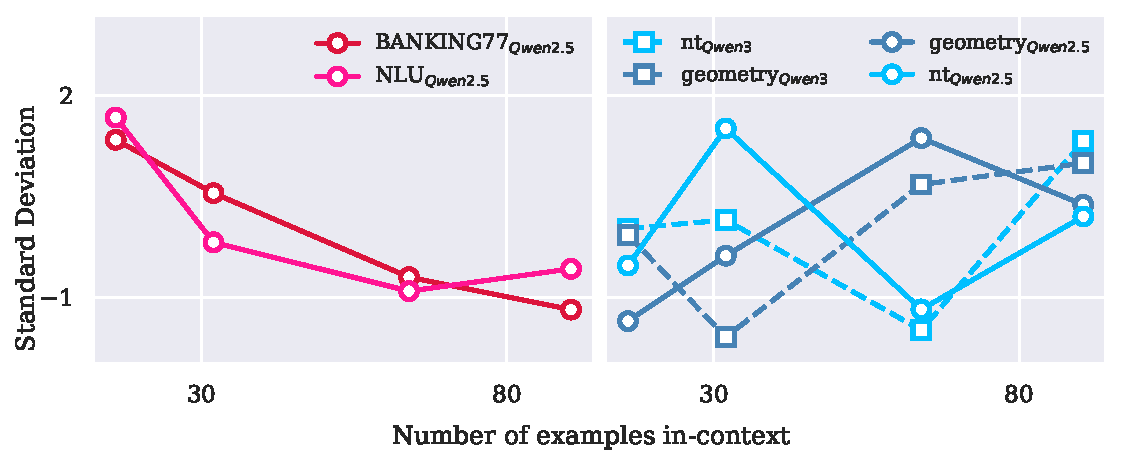
\includegraphics[width=\linewidth]{figures/standard_deviation.pdf}
    \caption{Standard deviation of performance across five random demonstration orders on classification tasks (\textcolor{orange}{warm colors}) versus reasoning tasks (\textcolor{Cerulean}{cool colors}), where nt corresponds to number\_theory. Results shown for Qwen2.5 (14B) (non-reasoning) and Qwen3 (14B) (reasoning).}
    \label{fig:std}
    \vspace{-3mm}
\end{figure}

If CoT demonstrations act as a learning signal rather than a static reference, their \emph{order} should matter, since order changes the trajectory of intermediate states induced by the context.
This prediction contrasts with findings on non-reasoning tasks, where order sensitivity decreases as the number of demonstrations grows~\cite{bertsch-etal-2025-context,baek2025revisitingincontextlearninglong}.

We quantify order sensitivity by sampling five random permutations of the same demonstration set and measuring the standard deviation of accuracy.
For non-reasoning tasks, we reproduce the low-variance behavior (Figure~\ref{fig:std}, left).
In contrast, for reasoning tasks we observe the opposite trend: variance \emph{increases} with more demonstrations (Figure~\ref{fig:std}, right).
This holds for both non-reasoning and reasoning LLMs.

Overall, many-shot CoT-ICL exhibits strong and growing path dependence: performance depends not only on \emph{which} demonstrations are provided, but also on \emph{how} they are sequenced.
This instability is consistent with CoT-ICL behaving as an in-context learning process whose effectiveness depends on the induced reasoning trajectory, motivating our in-context test-time learning perspective in the next section.
We further validate these conclusions by computing mean and standard deviation across five random demonstration-ordering seeds on an independently sampled ICL subset. The same qualitative trends persist for reasoning-oriented models, non-reasoning models, and cross-model CoT transfer, with full results in Appendix~\ref{sec:statistical_robustness}.


















